\section{Methode}
Zuerst soll die Kennlinie der Diode bestimmt werden. Dazu wird diese nach \cref{Aufbau} gemessen. Dabei wird die die Leistung der Mikrowellenstrahlung in Spannung umgewandelt. Dies wird auch in allen weiteren Messungen verwendet, da sich die Spannung einfacher direkt messen lässt.


\begin{figure}[h]
	\centering
	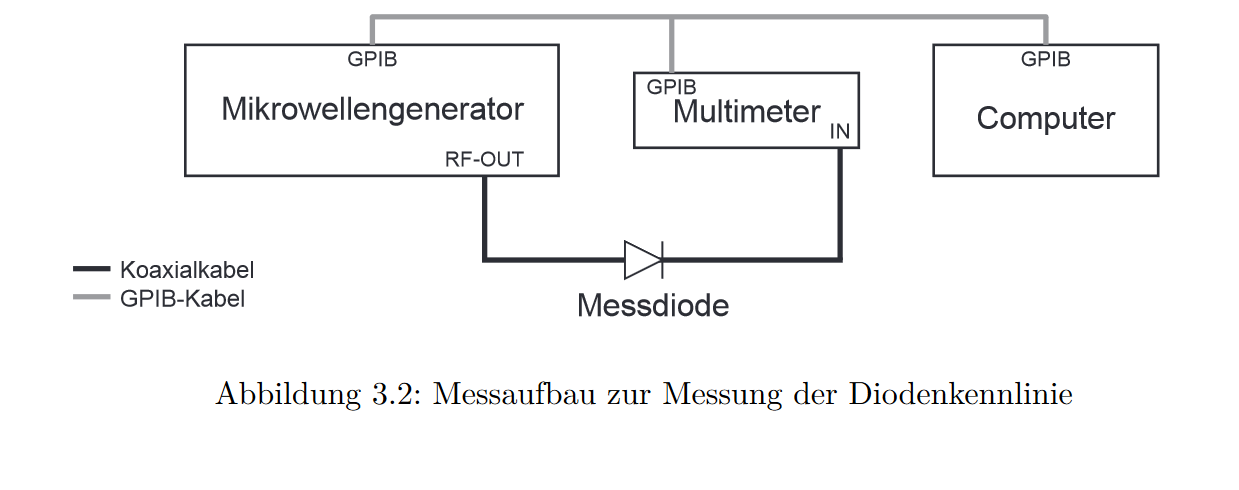
\includegraphics[scale=0.4]{../Diode_Aufbau.PNG}
	\caption{Skizze des Versuchaufbaus}
	\label{Aufbau}
\end{figure}

\section{Ergebnis}
Zuerst wird die Kennlinie der Diode bestimmt. Diese wird in \cref{fuck_scidavis} dargestellt. Dabei wird mit einer e-Funktion gefittet, durch die beschrieben wird, welche Leistung in wie viel Spannung umgewandelt wird. 

\begin{figure}[h]
	\centering
	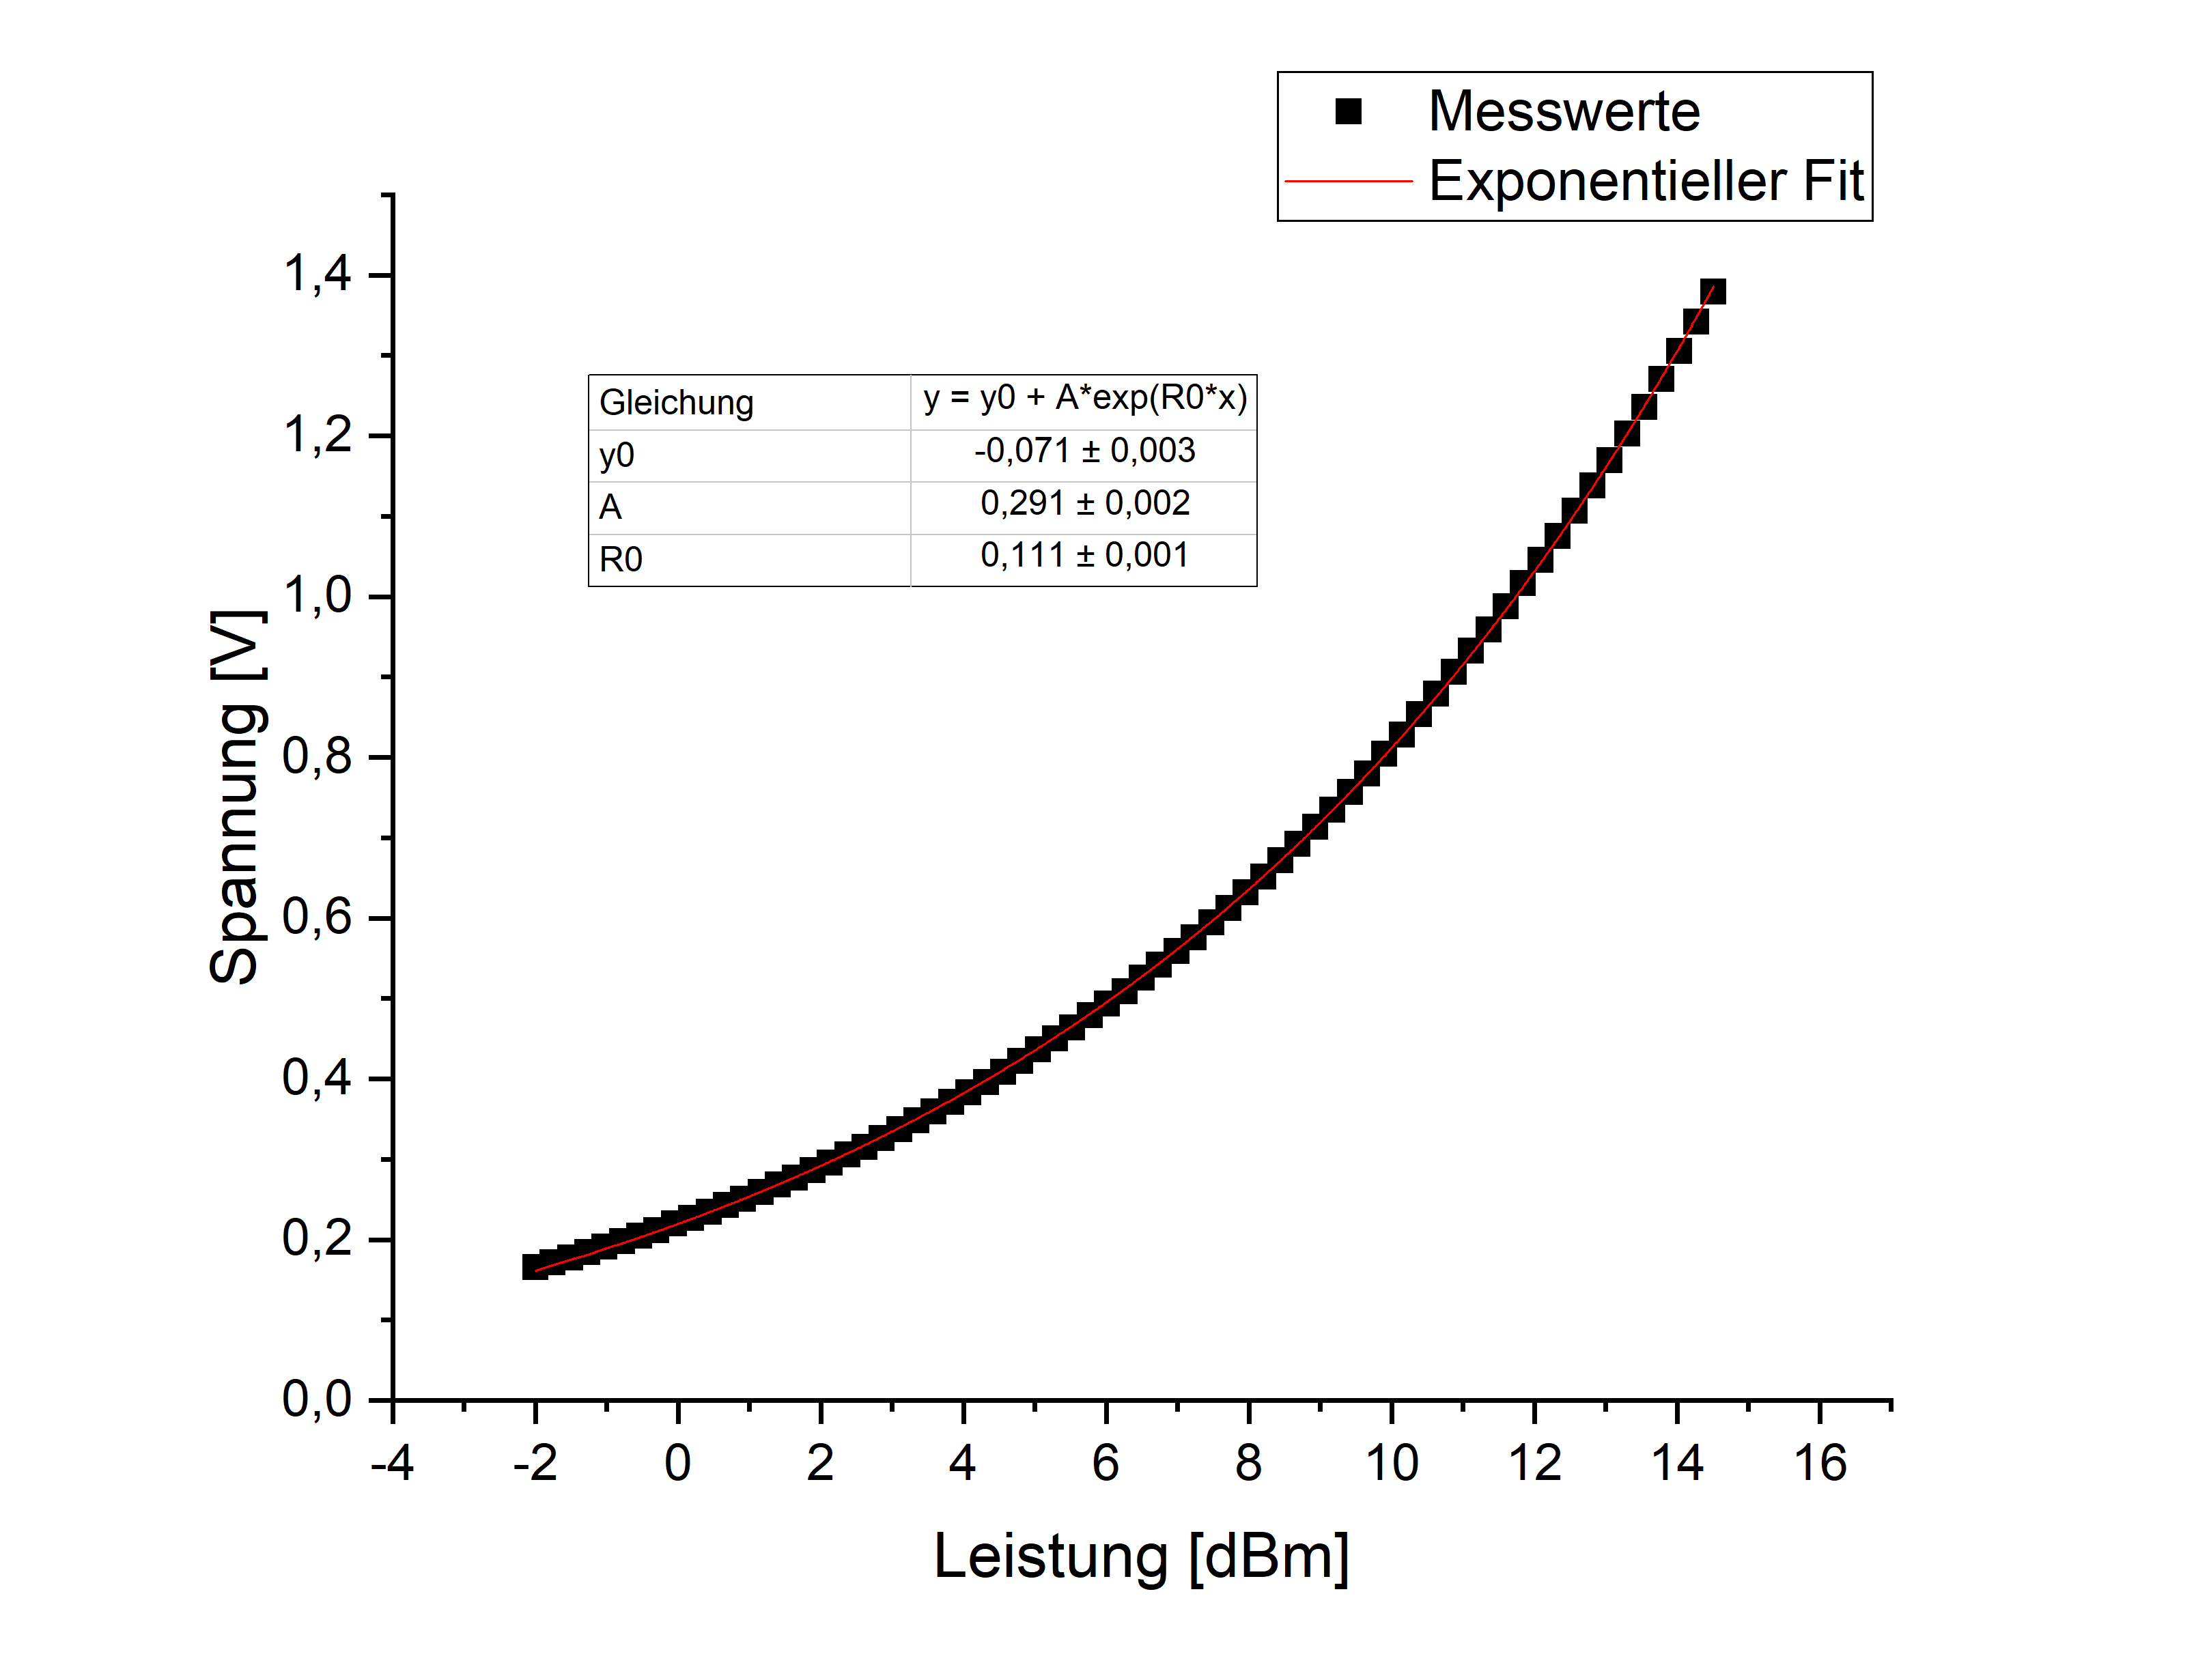
\includegraphics[scale=0.4]{../fuck_scidavis.png}
	\caption{Kennlinie der Diode}
	\label{fuck_scidavis}
\end{figure}